\documentclass{tstextbook}

% for lowercase roman enumerations
\usepackage{enumerate}

% define colors
\usepackage{xcolor}
\definecolor{mygreen}{rgb}{0,0.6,0}
\definecolor{mygray}{rgb}{0.5,0.5,0.5}
\definecolor{mymauve}{rgb}{0.58,0,0.82}

% languages listings
\usepackage{listings}
\lstdefinestyle{Pseudomath}
{
  basicstyle=\ttfamily,
  mathescape
}

\lstdefinestyle{Bash}
{
  language=bash,
  showstringspaces=false,
  %numbers=left,
  %numberstyle=\color{mygray}\textit,
  basicstyle=\footnotesize\ttfamily,
  %keywordstyle=\color{mygreen},
  %commentstyle=\color{mymauve},
  %identifierstyle=\color{blue},
  %stringstyle=\color{orange}
}

\lstdefinestyle{Python}
{
  language=Python,
  showstringspaces=false,
  numbers=left,
  numberstyle=\color{mygray}\textit,
  basicstyle=\footnotesize\ttfamily,
  keywordstyle=\color{mygreen},
  commentstyle=\color{mymauve},
  identifierstyle=\color{blue},
  stringstyle=\color{orange}
}




\begin{document}

\tsbook{Bitcoin Programming}
       {Konstantinos Karasavvas}
       {}
       {2020}
       {}{}{}
       {Version 0.1}
       {}
%       {Cover Designer}
%       {2017}
%       {xxxxx}{xxx--xx--xxxx--xx--x}{0.0}
%       {Publisher}
%       {City}

% Conventions
%---------------------------------------------------------------------------
% using emphbox to emphasize some text or a formula
% using note to NOTE something important
%---------------------------------------------------------------------------

%---------------------------------------------------------------------------
% Chapters
%---------------------------------------------------------------------------

% introduction
% to not include in ToC
%\section*{Preface}

\section{Preface}
This book is not about introducting what Bitcoin is. The readers are expected to understand the basics of the peer-to-peer network, what addresses and private keys are as well as have some experience using wallets and sending bitcoins\footnote{When we refer to the coins we will use \emph{bitcoin(s)} (lowercase `b') and when we refer to the protocol or the network we will use \emph{Bitcoin} (uppercase `B')}. The aim of this book is to help people delve deeper and in particular learn how to \emph{talk} to the Bitcoin network programmatically.

I started teaching Bitcoin programming in 2016. I have given hundreds of presentations in meetups or seminars and from 2017 higher education courses. Every year I was improving and updating my material to keep it as relevant as possible. Luckily, Bitcoin progresses at a steady pace while always keeping backwards compatibility. This is convenient because existing material will always be valid even though better alternatives might be introduced in the future.
  
To understand the material better myself and to improve the material in my courses I started an open source Python library, called bitcoin-utils\footnote{https://github.com/karask/python-bitcoin-utils}. The library was created for educational purposes and not for computational efficiency and that might be evident in certain parts of the implementation. Before starting this library I had investigated several other well-known Python libraries but I did not find an appropriate one for educational purposes. Some were too low-level with limited documentation while others where abstracting concepts that I deemed where important for students to understand.

This book is about teaching Bitcoin programming. Throughout the years I have prepared a lot of material based on my early code experiments, the bitcoin-utils library and several online resources, especially the Bitcoin Stack Exchange\footnote{https://bitcoin.stackexchange.com/} and the excellent Bitcoin Book\footnote{https://github.com/bitcoinbook/bitcoinbook} by A. Antonopoulos. While I try to always credit the initial sources that I have consulted over the years it is very possible that I have missed some. Please let me know and I will update accordingly.

My hope is that this book consolidates all this teaching material with practical examples so as to help others understand Bitcoin programming. 

I have been using a Linux-based machine and thus most command-line examples are from \pyth{bash} shell. However, people comfortable with other Operating Systems should have no issues to adjust as needed.

\chapter{How Bitcoin Works}
\label{ch:howbitcoinworks}

\begin{summary}
This chapter provides a high-level introduction of how Bitcoin works. It aims to be a summary of the prerequisite knowledge required by the reader before moving into the following chapters. The operation of the Bitcoin network is demonstrated with a walkthrough of a transaction and its journey from its creation up until its final destination, the Bitcoin blockchain.
\end{summary}

\section{The Story of a Transaction}
Transactions specify the transfer of bitcoin ownership. Assume we have three actors; Zed, Alice and Bob. Zed has sent 1.5 bitcoins to Alice with $TX_x$ and Alice wants to send 1 bitcoin to Bob. The transaction history will already have an entry of how Alice got her bitcoins (e.g. from Zed).

\begin{note}
Internally, the Bitcoin protocol operates with satoshis: $1~satoshi = 0.00000001~BTC$. Thus, when we want to transfer 1 BTC we actually transfer $100000000~satoshis$.
\end{note}

To send 1 bitcoin (or \emph{BTC}) Alice needs to create a transaction $TX_y$ that sends 1 BTC to Bob. We know that Alice has at least 1.5 BTC from $TX_x$.

\begin{emphbox}
\begin{lstlisting}[style=Pseudomath]
    $TX_x$: 1Zed transfers 1.5 BTC to 1Alice
    $TX_y$: 1Alice transfers 1 BTC to 1Bob
\end{lstlisting}
\end{emphbox}

The names 1Zed, 1Alice and 1Bob are short for the actual bitcoin addresses of Zed, Alice and Bob respectively. So Alice will send 1 BTC from her 1Alice bitcoin address to Bob to his 1Bob address.

Alice has to prove that she is indeed the owner of the address 1Alice when she creates the $TX_y$. Bob does not need to do anything to receive the bitcoins.

A transaction can consist of several \emph{inputs} (outputs of past transactions) and several \emph{outputs} (addresses to send bitcoins to). When an input is used it is completely consumed; i.e. all the bitcoins that the TX contains as inputs need to be \emph{spent}.

\begin{figure}[h]
\begin{center}
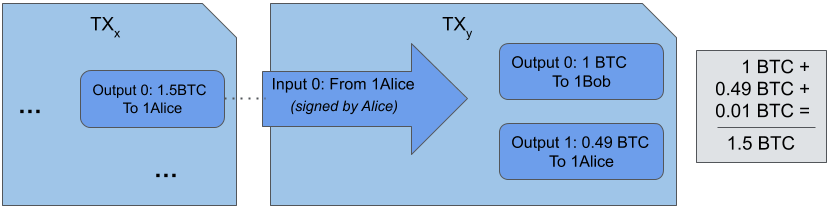
\includegraphics[scale=0.5]{images/typical-transaction}
\caption{Typical one input two outputs transaction.}
\label{fig:typical-transaction}
\end{center}
\end{figure}

The amount of all the inputs needs to be greater or equal to the amounts of outputs. If greater (recommended) the difference is an implied transaction fee that goes to the miners (see figure~\ref{fig:typical-transaction} where the miner receives 0.01 BTC). A typical transaction transfers some bitcoins to another user and returns the remaining bitcoins as change to the originating address or another address that the sender controls.

\begin{note}
For privacy reasons it is recommended to send the change to a different address than the originating. Most bitcoin wallets already do this behind the scenes.
\end{note}

Any number of inputs and outputs is possible as long as a transaction fee is included; the larger the transaction the larger the transaction fee. The unspent outputs are called \emph{Unspent Transaction Outputs (UTXOs)} and the set of UTXOs is essentially all the available bitcoins in the network.

Once a transaction is created it needs to be sent to a Bitcoin node. After the node receives the transaction it checks if it is valid, e.g. the output amounts should be less or equal to the input amounts, the signature proving ownership should be valid, etc. If it is valid the node will propagate it to all its peers\footnote{To be more precise they will notify their peers of the transaction by its \emph{transaction identifier (txid)} and the peers can choose to request it or not. More details will be provided in the Peer-to-Peer chapter.}, i.e. the other nodes that it is aware of. In turn, the other nodes will check if the transaction is valid and so on and so forth until all nodes receive the transaction (see figure~\ref{fig:transaction-propagation}).

\begin{figure}[h]
\begin{center}
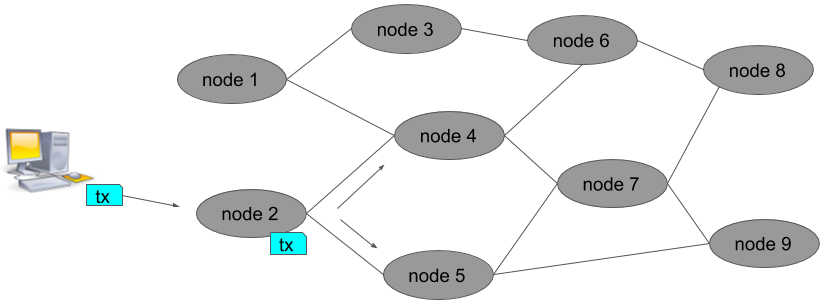
\includegraphics[scale=0.5]{images/transaction-propagation}
\caption{Example of transaction propagation through the network.}
\label{fig:transaction-propagation}
\end{center}
\end{figure}


\section{From Transactions to Blocks}
From a Bitcoin's node perspective, the node receives transactions and places all valid ones into its memory pool, or \emph{mempool}. It keeps receiving new ones until it decides that it will group some of those transactions into a block (see figure~\ref{fig:node-perspective}).

\begin{figure}[h]
\begin{center}
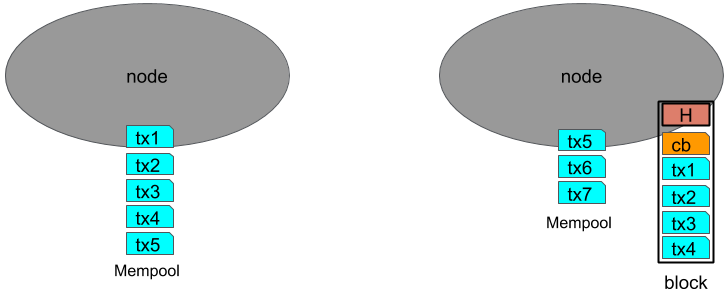
\includegraphics[scale=0.5]{images/node-perspective}
\caption{A node receives transactions into its mempool and can attempt to create new blocks for the network.}
\label{fig:node-perspective}
\end{center}
\end{figure}

%\vspace{3em}
\begin{note}
We are describing what mining nodes typically do. The majority of nodes are not mining nodes and thus do not attempt to create new blocks, rather they validate and propagate valid transactions and blocks when they are aware of them.
\end{note}

Every block contains a \emph{coinbase} transaction that is added by the miner (see next section) and it sends a deterministically calculated reward to an address of the miner's choosing. Finally a header is added to the block containing important information that links this block to its parent and other information that we will examine in the next section.

\section{Mining: basics}
After a node creates a block it will attempt to make it final by propagating it to all other nodes in the network. Multiple nodes will receive the same transactions and will create blocks; nodes choose which TXs to include (see figure~\ref{fig:different-nodes-mining}). They can create and propagate a block at any time.

\begin{emphbox}
But how do we select which blocks will be part of the blockchain? Since, miners include a reward for themselves everyone wants their block to be the next block in the blockchain. In other words, how do we avoid spam and Denial of Service (DoS) attacks?
\end{emphbox}

For a block to be considered valid a miner has to prove that he has done some intensive computational work. Thus, miners have to spend resources before they create a block. This mechanism of proving computational work is called \emph{Proof-of-Work (PoW)} and it involves solving a problem or puzzle. PoW puzzles have the fundamental property of being difficult to solve but trivial to validate their correctness. 

Bitcoin mining is the process of solving the PoW puzzle and selecting the next valid block in a way that is undisputed and thus achieve consensus on the current blockchain state. Bitcoin uses the Hashcash PoW algorithm~\cite{Back2002-hashcash} for its mining.

\begin{figure}[h]
\begin{center}
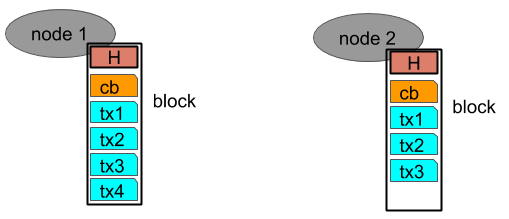
\includegraphics[scale=0.5]{images/different-nodes-mining}
\caption{All nodes will eventually receive all transactions but they are free to include them into a block as they see fit.}
\label{fig:different-nodes-mining}
\end{center}
\end{figure}

The Proof-of-Work puzzle is to compute a cryptographic hash (effectively a big hexadecimal number) of the new block that we want to create which should be less than a target number. The target number that the hash needs to be less than can be deterministically calculated by all nodes and is such that it would take around 10 minutes to calculate with the current network processing power, also called hashing power. Since a hash is random it will take several attempts to find a proper hash but other nodes will verify with only one attempt.

\begin{note}
A cryptographic hash function is a hash function that takes an arbitrary block of data and returns a fixed-size bit string, the cryptographic hash value, such that any (accidental or intentional) change to the data will also change the hash value significantly.
\end{note}

As more miners join the blocks will be created faster so the puzzle’s difficulty automatically adjusts (increases) so that it again requires approximately 10 minutes to solve. This \emph{difficulty adjustment} is happening every 2016 blocks, which is approximately 2 weeks if each block takes 10 minutes to mine.

The hash algorithm used is \keyword{SHA256} and it is applied twice to the block header. As we will see later the header uniquely represents the whole block including all the transactions and thus hashing the header is effectively the same as hashing the whole block, but much more efficiently since the header is much smaller.

\begin{emphbox}
\begin{lstlisting}[style=Pseudomath]
SHA256( SHA256( block_header ) )
\end{lstlisting}
\end{emphbox}

The miner that successfully creates a valid block first will get the bitcoin reward that they have set themselves in the coinbase transaction as well as the fees from all the transactions in the block.

The block reward can be deterministally calculated according to the current \emph{block height}. The reward started at 50 bitcoins and is halved every 210000 blocks (approximately 4 years for 10 minute blocks). So, after block 630000 the reward will be 6.25 bitcoins. The mining reward can be claimed by the miner only after 100 \emph{confirmations}, i.e. after 100 blocks have been confirmed as part of the blockchain since.


\section{Mining: a bit more technical}
\label{sec:mining-technical}

The structure of the block header is as follows:

\begin{center}
\begin{tabular}{ |l|l|l| }
\hline
	Field & Description & Size (bytes)\\
\hline
	version        & Block version number                               & 4\\
	hashPrevBlock  & 256-bit hash of the previous block                 & 32\\
	hashMerkleRoot & 256-bit hash representing all the TXs in the block & 32\\
	timestamp      & Seconds since 1970-01-01T00:00 UTC                 & 4\\
	target (bits)  & The target that the hash should be less than       & 4\\
	nonce          & 32-bit number                                      & 4\\
\hline
\end{tabular}
\end{center}

Block version and timestamp are self explanatory but we will briefly go through the remaining fields.

\subsection*{hashMerkleRoot}
A block has two parts, the header and the transactions. Since we only hash the block header to link blocks together, a header needs to represent the whole block, including all its transactions (coinbase and normal). The transactions are indirectly hashed via using a merkle root and being included in the block by \keyword{hashMerkleRoot}.

A merkle tree\footnote{https://en.wikipedia.org/wiki/Merkle\_tree} is constructed by concatenating all the transaction hashes, in pairs. The resulting hashes are again concatenated and hashed until only a single hash remains, the merkle root.

\begin{figure}[h]
\begin{center}
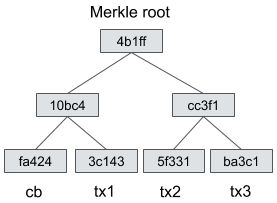
\includegraphics[scale=0.5]{images/merkle-tree}
\caption{Simple merkle root calculation of coinbase and three transactions.}
\label{fig:merkle-tree}
\end{center}
\end{figure}

An important property of a merkle tree is that you can efficiently prove that a hash (and thus transaction) is part of the merkle root. A merkle proof consists of the hashes required to reconstruct the merkle root from the leaf TX, thus proving that the TX hash is indeed part of the merkle tree. For example to prove that \keyword{tx1} is part of the merkle root we would need to provide the hash of \keyword{cb} and its positioning (i.e. left) as well as the parent hash of \keyword{tx2} and \keyword{tx3} (\keyword{cc3f1}) and its positioning (i.e. right).

\subsection*{hashPrevBlock}
This is the hash of the previous block in the blockchain. It designates the parent of the current block and it is effectively what chains the blocks together. For example, if someone changes a transaction in the previous block then the \keyword{hashPrevBlock} will change. This is of particular importance as we will see in more detail in section~\ref{sec:blocks-nakamote-consensus}.

\subsection*{target}
Target bits or just bits is represented as an 8 hex-digit number. The first 2 digits are the exponent and the rest the coefficient. Target bits can be used to calculate the actual target with the following formula:

\begin{emphbox}
\begin{lstlisting}[style=Pseudomath]
    $target = coefficient * 2^{(8 * (exponent - 3))}$
\end{lstlisting}
\end{emphbox}

The highest possible target (the easiest target) is defined as \keyword{0x1d00ffff} and gives a 32-byte target of (expressed as a 64 hexadecimal number):

\small
\begin{emphbox}
\begin{lstlisting}[style=Pseudomath]
0x00000000ffff0000000000000000000000000000000000000000000000000000
\end{lstlisting}
\end{emphbox}
\normalsize

In Python that would be calculated as follows:
\vspace{1em}
\begin{lstlisting}[style=Python,label={lst:encodings-1},caption={Python examples},captionpos=b]
>>> 0x00ffff * 2**(8*(0x1d - 3))
26959535291011309493156476344723991336010898738574164086137773096960
>>> format(26959535291011309493156476344723991336010898738574164086137773096960, '064X')
'00000000FFFF0000000000000000000000000000000000000000000000000000'
\end{lstlisting}
\vspace{1em}



If the result of hashing the block header produces a hash that begins with 0x00000000e (or less) then we have found a solution. That would require, statistically ~$2^{32}$ (4,294,967,296) attempts on average. The smaller the target the more difficult the solution, the more attempts on average.

Another representation of target, easier for humans to understand, is \emph{difficulty} which represents the ratio between the highest target and the current target:

\begin{emphbox}
\begin{lstlisting}[style=Pseudomath]
$Difficulty = \dfrac{highest\_target} {current\_target}$
\end{lstlisting}
\end{emphbox}

When Bitcoin started it started with the highest target (\keyword{0x1d00fff}) and thus it had difficulty 1. Difficulty 1 requires $2^{32}$ attempts on average to find a solution. Difficulty 10 requires $2^{32} * 10$ attempts on average, etc.

\subsection*{nonce}
The nonce is just a number used to differentiate the hash while trying to reach the target. Given that it is only 4 bytes it can only handle ~4.2 billion combinations, while we need quintillion nowadays\footnote{As of August 2020.}.

When the limit was reached miners started modifying the timestamp (e.g. -1 sec) to allow for an additional of ~4.2 billion combinations. However, there is a limit of seconds that a node can deviate from the rest of the network so that did not suffice either\footnote{The timestamp must be higher than the median of the 11 immediate ancestors of the block and higher than the timestamp of its parent. Finally, the timestamp must be no more than 2 hours in the future.}.

Finally, miners started to use the unused space of coinbase's transaction input as an extra nonce allowing an immense amount of extra nonces to be used\footnote{The size of the coinbase input can be from 2 to 100 bytes.}. 


\subsection*{Difficulty Adjustment}
We already mentioned that the difficulty to find the proper hash is expected to take approximately 10 minutes. However, Bitcoin is an open system and anyone can join (or leave) the network as a miner. Thus, the network’s hashrate can increase (or decrease) with time. 

With more hashing power blocks will be issued faster than 10 minutes and thus the network has to adjust the difficulty of the problem accordingly. This can be seen in figure~\ref{fig:hashrate-difficulty}.

\begin{figure}[h]
\begin{center}
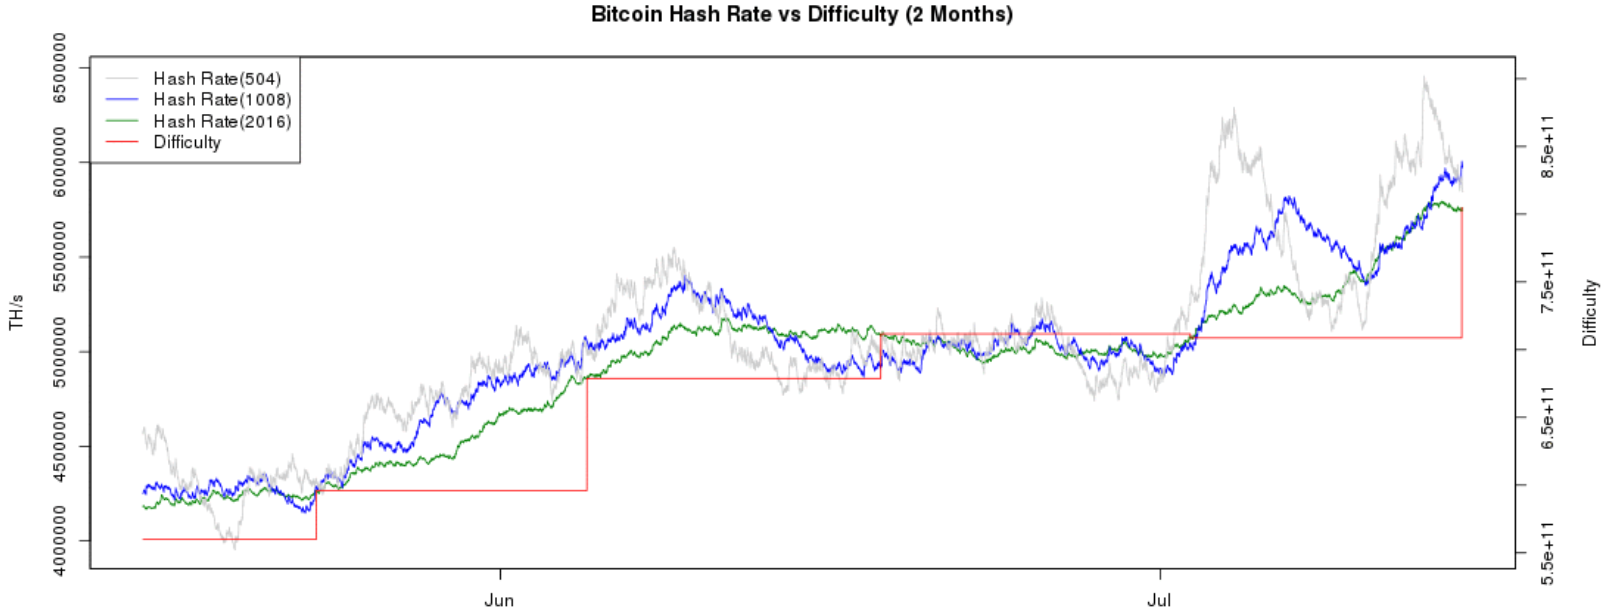
\includegraphics[scale=0.25]{images/hashrate-difficulty}
\caption{Hashrate and difficulty adjustment.}
\label{fig:hashrate-difficulty}
\end{center}
\end{figure}

Specifically, Bitcoin nodes, check every 2016 blocks ($\sim$2 weeks) the timestamps between consecutive blocks and sums them to find out how much time $t$ it took. We want $t$ to take two weeks and thus the new difficulty will be:

\begin{emphbox}
\begin{lstlisting}[style=Pseudomath]
$old\_difficulty * ( \frac{2\_weeks} {t} )$
\end{lstlisting}
\end{emphbox}

\subsection*{Mining Process in a nutshell}
Here we describe a mining node's actions for mining in a simplified step by step process:

\begin{enumerate}
\item Gather valid TXs into blocks
\item Get the longest chain’s top block hash and add it in hashPrevBlock
\item Add timestamp, nonce and extra nonce in the first TX (coinbase)
\item Calculate the merkle root of valid TXs and add it to hashMerkleRoot
\item Hash the header to find a solution smaller than the specified target
  \begin{itemize}
  \item modify timestamp, nonce or extra nonce as appropriate
  \item rehash until a solution is found or the longest chain changed
  \end{itemize}
\end{enumerate}

During the above process:
\begin{itemize}
\item If more TXs are included in the block or the extra nonce is modified
  \begin{itemize}
  \item recalculate merkle root and update it
  \end{itemize}
\item If the longest chain changed we want to build on that chain from now on
  \begin{itemize}
  \item update the valid TX set
  \item update the timestamp
  \item recalculate the merkle root
  \item use the new block as hashPrevBlock
  \end{itemize}
\end{itemize}


\section{The story of a Block}
\label{sec:blocks-nakamote-consensus}
Once a node finds a solution to the PoW problem it will propagate it to its peers. They will check if the block (and every transaction) is valid and if it is they will propagate it to all their peers\footnote{To be more precise they will notify their peers of the block and the peers can choose to request the actual block or not. More details will be provided in the Peer-to-Peer chapter.}. In turn, the peers will check again for the solution as well as the block validity and they will propagate again and so on and so forth until all nodes receive the new block (see figure~\ref{fig:block-propagation}).

\begin{figure}[h]
\begin{center}
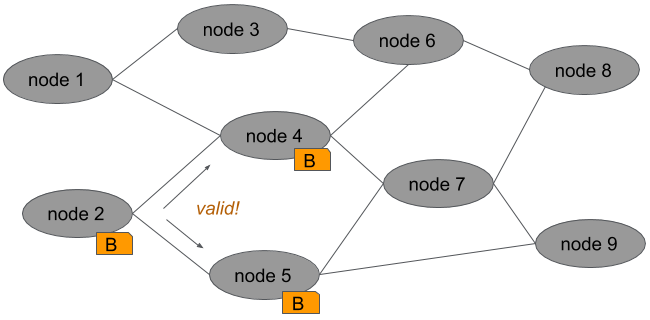
\includegraphics[scale=0.5]{images/block-propagation}
\caption{Example of block propagation through the network.}
\label{fig:block-propagation}
\end{center}
\end{figure}

The new block is being added on top of the existing blocks (every ~10 minutes). This occurs on every single node on the network thus the blocks are the same in all nodes. Blocks are linked with cryptographic hashes forming a chain of blocks, called \emph{Blockchain}.

When Block \keyword{B1} is accepted by the network we say that a transaction on that block has one confirmation. When \keyword{B3} is accepted we say that our transaction has 3 confirmations (see figure~\ref{fig:node-perspective-2}. The more confirmations the more final and secure a transaction is. 

\begin{figure}[h]
\begin{center}
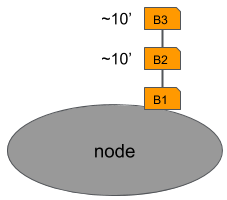
\includegraphics[scale=0.5]{images/node-perspective-2}
\caption{A node receives blocks and links them to form the blockchain.}
\label{fig:node-perspective-2}
\end{center}
\end{figure}


\section{Nakamoto Consensus and Trust}
Each node receives blocks and builds its own blockchain in isolation. A fundamental innovation that bitcoin introduced is the Nakamoto consensus, i.e. how do different nodes come to agreement on what is the current state of the blockchain.

If two miners find a block (almost) at the same time then network peers will get a different block first. They will then start building the next block based on the one they received first. That means that the network at that time has two possible states.

In Nakamoto consensus the basic rule is that miners should \emph{follow the longer chain} (the one with the most computation). Thus, when one of the miners finds the next block all miners will choose the longer chain and consensus is achieved. For an example see the different steps in figure~\ref{fig:nakamoto-consensus}.

\begin{figure}[h]
\begin{center}
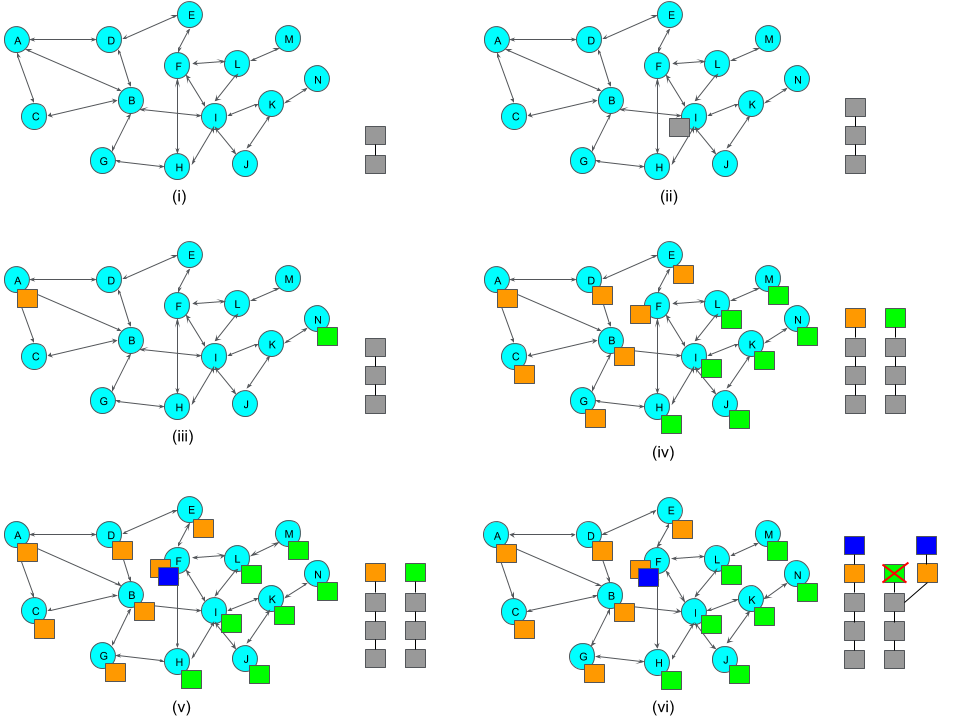
\includegraphics[scale=0.4]{images/nakamoto-consensus}
\caption{Nakamoto Consensus example.}
\label{fig:nakamoto-consensus}
\end{center}
\end{figure}

\begin{enumerate}[(i)]
\item Initially our example network has only two blocks and all nodes are in sync.
\item Then node \keyword{I} finds the next block, which is disseminated to all other nodes and again everyone is in sync.
\item Next, let's suppose that two nodes find a solution at about the same time. These blocks will typically be very similar, including almost the same transactions, but will be different.
\item The nodes will propagate their blocks and some peers will get one of the blocks and some the other. The nodes are aware of both blocks but they will use the block that they received first as the next block and will start mining the next block on top of that block. At this stage we do not have consensus since some of the nodes have a blockchain with the orange block at the top and some the green block.
\item However, after a while a new block will be found. In our example, this is node \keyword{F} and it will propagate it throughout the network.
\item Finally, when the block is propagated to the nodes with the green block on top they will realise that there is a longer chain than the one that they are working on. According to nakamoto consensus the nodes will accept the longer chain as the \emph{valid} chain and ignore the green block. The green block is typically called an \emph{orphan} block\footnote{Precise terminology is more complicated as discussed in https://bitcoin.stackexchange.com/questions/5859/what-are-orphaned-and-stale-blocks}. And now all nodes are in sync again. 
\end{enumerate}

\vspace{3em}
\begin{note}
If there are transactions in the orphaned block that are not in the orange or the blue block they are moved to the mempool ready to be included in one of the following blocks.
\end{note}

Of course it would be possible that at step (v) 2 new solutions could again be found one from a node with an orange block on top and another from a green block on top. Similarly, consenus would be achieved with the following block and two blocks would be orphaned. In such a case, we would say that a 2-block \emph{reorg} occurred.

Nakamoto consensus is a natural and expected reorg event that currently occurs less than once per month\footnote{https://bitcoinchain.com/block\_explorer/orphaned} even for 1-block reorgs. The chance of a reorg is proportional with the number of blocks and thus larger reorgs are exceedingly rare.

\subsection*{Establishing Trust}
As we have seen, blocks are linked together by including the hash of the previous block on the new block. For example, in figure~\ref{fig:blockchain-trust} the hash of \keyword{B1} is included in the header of \keyword{B2}.

\begin{figure}[h]
\begin{center}
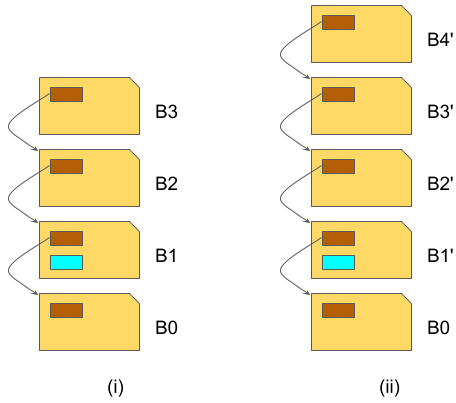
\includegraphics[scale=0.5]{images/blockchain-trust}
\caption{Linked blocks and Trust.}
\label{fig:blockchain-trust}
\end{center}
\end{figure}

In our example a transaction in \keyword{B1} (represented with the cyan box) has 3 confirmations. If an attacker wishes to attempt a double spend attack\footnote{https://en.wikipedia.org/wiki/Double-spending} they will need to create and new \keyword{B1'} block with the modified transaction. However, there are two more blocks on top of \keyword{B1} and thus the attackers block will be ignored since \keyword{B1'} will not be the longer chain. The attacker also needs to create \keyword{B2'}, \keyword{B3'} and \keyword{B4'} to succeed in a double spend. 

To achieve that, the attacker will need to have the majority of the network's hash rate, which is what is typically called the 51\% attack\footnote{Certain attacks, like selfish mining, could be successful with a smaller percentage.}.

Achieving this kind of hash rate and sustaining it would require extravagant amounts of funds to accommodate for the mining hardware and operational costs and thus it would not be easily feasible. 

This is even more evident when one considers what is possible with such an attack: potential censorship and double spends. Even with such an attack the funds on all the Bitcoin addresses are safe as is the historical records of the transactions; the former are secured by strong cryptography while the latter would require much more hash rate to modify them.

Bitcoin security model is based on game theory principles and proper incentives. Economically speaking only a very irrational entity would make such an attack since setting up the environment for the attack would position the attacker in a very economically advantageous position, i.e. they will be earning a lot of money with the mined bitcoins.

\begin{note}
Even though Bitcoin and Nakamoto Consensus provide us with some of the strongest probabilistic guarantees it is theoretically possible to be influenced by malevolent actors. 
\end{note}

Until now the network had been extremely resilient to any kind of attack and has proven its robustness and stability securing hundreds of billions worth of value. The Bitcoin blockchain is considered by many as the most immutable structure constructed by humans.


\section{Basic interaction with a node}
After installing the Bitcoin software\footnote{You can find several online resources on how to install Bitcoin specifically for your operating system. Such tutorial is outside the scope of this book.} we can notice that it includes several executables, one providing the core functionality and the other for interaction and extra utility:
\begin{description}
	\item[bitcoind:] The daemon server that implements the Bitcoin protocol and networking functionality. It also includes a wallet. It provides a JSON-RPC API to talk to the node (ports: mainnet: 8332, testnet: 18332, regtest: 18443, sigtest: 38332).
	\item[bitcoin-cli] Provides a command-line interface to \emph{talk} to the daemon server.
	\item[bitcoin-qt] Provides a graphical user interface to the Bitcoin peer and wallet (subset of the API as part of GUI but also provides a console for all calls).
	\item[bitcoin-tx] Allows to create, parse or modify transactions.
	\item[bitcoin-wallet] Allows to create, parse or modify transactions.
\end{description}

\subsection*{Bitcoin software configuration and development environments}
The configuration file is bitcoin.conf and its default location depends on the operating system used (e.g. in linux system it is located at ~/.bitcoin/bitcoin.conf). Some important options for development and testing\footnote{https://developer.bitcoin.org/examples/testing.html} your application include:

\begin{description}
	\item[deamon=1] Runs the Bitcoin node in the background.
	\item[server=1] Allows JSON-RPC commands but only from localhost.
	\item[testnet=1] The Bitcoin node uses the testnet network for development (i.e. fake funds). If the option is missing or if it is `0' then mainnet (the real network) is used.
	\item[regtest=1] This is a local test environment. The blockchain starts at height 0 (genesis block) and we can trivially mine new blocks with the \keyword{generatetoaddress} command. This allows developers to also control the block creation and get fake funds immediately. Regtest uses testnet’s network parameters (e.g. address prefixes, etc).
	\item[signet=1] New test network for development that adds an additional signature requirement for block validation. Signet is similar in nature to testnet, but more reliable and centrally controlled. Anyone can run their own unique signet for their testing purposes. Available from Bitcoin Core v0.21.0.
	\item[addnode=12.34.56.78] Also connect to specific peer (multiple \keyword{addnode}'s can be used). If no network is specified it will only apply to mainnet.
	\item[connect=12.34.56.78] Only connect to specific node (multiple \keyword{connect}'s can be used). If no network is specified it will only apply to mainnet.
	\item[rpcallowip=12.34.56.78] Allows JSON-RPC connections from this IP (default is localhost).
	\item[prune=1000] Only keep more recent blocks that fit in 1000 MiB. Pruning is not compatible with \keyword{txindex} and \keyword{rescan}. 
	\item[mempoolsize=100] Only keep transactions that fit in 100 MiB. Transactions are ordered by fee rate and if there is not enough space the ones with the lowest fee rate are removed.
\end{description}

We can also include sections like \keyword{main}, \keyword{test} and \keyword{regtest} to provide specific options depending on the network used. Usually, when optioins are not specified under a section they apply to all sections with the exception of \keyword{addnode}, \keyword{connect}, \keyword{port}, \keyword{bind}, \keyword{rpcport}, \keyword{rpcbind} and \keyword{wallet}.

A typical minimalistic config for development is:
\begin{emphbox}
\begin{lstlisting}[style=Bash]
daemon=1
testnet=1
#regtest=1

server=1
rpcuser=kostas
rpcpassword=toodifficulttoguess

[main]
mempoolsize=300

[test]
mempoolsize=100

[regtest]
mempoolsize=20
\end{lstlisting}
\end{emphbox}


\subsection*{Examples of Calls using \keyword{bitcoin-cli}}


To get help of all available commands and how to get further help:
\begin{emphbox}
\begin{lstlisting}[style=Bash]
$ bitcoin-cli help
\end{lstlisting}
\end{emphbox}
\vspace{1em}

After version 0.22 a bitcoin wallet is not created by default. We have to create one ourselves. We can create a default wallet with:

\begin{emphbox}
\begin{lstlisting}[style=Bash]
$ bitcoin-cli -named createwallet wallet_name="testwallet" load_on_startup=true
\end{lstlisting}
\end{emphbox}
\vspace{1em}

\noindent The default wallet is a descriptor wallet (see chapter~\ref{ch:keys-and-addresses} for more on descriptor wallets). To use commands like \keyword{importaddress} and \keyword{dumpprivkey} a non-descriptor wallet needs to be created:

\begin{emphbox}
\begin{lstlisting}[style=Bash]
$ bitcoin-cli -named createwallet wallet_name="testwallet-2" descriptors=false
\end{lstlisting}
\end{emphbox}
\vspace{1em}



\noindent To get the current block height:
\begin{emphbox}
\begin{lstlisting}[style=Bash]
$ bitcoin-cli getblockcount
1806981
\end{lstlisting}
\end{emphbox}
\vspace{1em}

\noindent To get the current balance of all addresses:
\begin{emphbox}
\begin{lstlisting}[style=Bash]
$ bitcoin-cli getbalance
1.51815479
\end{lstlisting}
\end{emphbox}
\vspace{1em}

\noindent To get a new legacy\footnote{The typical P2PKH Addresses starting with \keyword{1} on mainnet and \keyword{m} or \keyword{n} on testnet.} address:
\begin{emphbox}
\begin{lstlisting}[style=Bash]
$ bitcoin-cli getnewaddress "" legacy
mvBGdiYC8jLumpJ142ghePYuY8kecQgeqS
\end{lstlisting}
\end{emphbox}
\noindent By default Bitcoin v0.20+ use \keyword{bech32} (or native segwit) addresses. The example above overrides the default. We will examine the different kind of Bitcoin addresses in Chapter~\ref{ch:keys-and-addresses}.
\vspace{1em}

\noindent To encrypt the wallet with a passphrase:
\begin{emphbox}
\begin{lstlisting}[style=Bash]
$ bitcoin-cli walletencrypt PaSsPhRaSe
wallet encrypted; Bitcoin server stopping, restart to run with encrypted 
wallet. The keypool has been flushed and a new HD seed was generated (if 
you are using HD). You need to make a new backup.
\end{lstlisting}
\end{emphbox}
\vspace{1em}

\noindent To unlock an encrypted wallet for 2 minutes to spend funds:
\begin{emphbox}
\begin{lstlisting}[style=Bash]
$ bitcoin-cli walletpassphrase PaSsPhRaSe 120
\end{lstlisting}
\end{emphbox}
\vspace{1em}

\noindent To create a wallet backup:
\begin{emphbox}
\begin{lstlisting}[style=Bash]
$ bitcoin-cli backupwallet wallet.backup
\end{lstlisting}
\end{emphbox}
\vspace{1em}

\noindent To import a backed up wallet:
\begin{emphbox}
\begin{lstlisting}[style=Bash]
$ bitcoin-cli importwallet wallet.backup
\end{lstlisting}
\end{emphbox}
\vspace{1em}

\noindent To get the node's networking info:
\begin{emphbox}
\begin{lstlisting}[style=Bash]
$ bitcoin-cli getnetworkinfo
{
  "version": 200000,
  "subversion": "/Satoshi:0.20.0/",
  "protocolversion": 70015,
  "localservices": "0000000000000409",
  "localservicesnames": [
    "NETWORK",
    "WITNESS",
    "NETWORK_LIMITED"
  ],
  ... 
}
\end{lstlisting}
\end{emphbox}
\vspace{1em}

\noindent To get the node's blockchain info:
\begin{emphbox}
\begin{lstlisting}[style=Bash]
$ bitcoin-cli getblockchaininfo
{
  "chain": "test",
  "blocks": 1887283,
  "headers": 1887283,
  "Bestblockhash": "0000000000074e...9d44e05b4",
  "difficulty": 1420477.254893854,
  "mediantime": 1604662239,
  "verificationprogress": 0.9999999194957088,
  "initialblockdownload": false,
  "chainwork": "000000000000...a2762e8",
  "size_on_disk": 28640545955,
  "pruned": false,
  ...
}
\end{lstlisting}
\end{emphbox}
\vspace{1em}

\noindent To get the node's mining info:
\begin{emphbox}
\begin{lstlisting}[style=Bash]
$ bitcoin-cli getmininginfo
{
  "blocks": 1887283,
  "difficulty": 1420477.254893854,
  "networkhashps": 131251268159888.9,
  "pooledtx": 9,
  "chain": "test",
  "warnings": "Warning: unknown new rules activated (versionbit 28)"
}
\end{lstlisting}
\end{emphbox}
\vspace{1em}

\noindent To get the node's wallet info:
\begin{emphbox}
\begin{lstlisting}[style=Bash]
$ bitcoin-cli getwalletinfo
{
  "walletname": "wallet-test1",
  "walletversion": 169900,
  "format": "bdb",
  "balance": 0.00065838,
  "unconfirmed_balance": 0.00000000,
  "immature_balance": 0.00000000,
  "txcount": 1,
  "keypoololdest": 1667229693,
  "keypoolsize": 1000,
  "hdseedid": "c41632b90911bb4d4b172190bf9a27def9535fc4",
  "keypoolsize_hd_internal": 1000,
  "paytxfee": 0.00000000,
  "private_keys_enabled": true,
  "avoid_reuse": false,
  "scanning": false,
  "descriptors": false,
  "external_signer": false
}
\end{lstlisting}
\end{emphbox}
\vspace{1em}


\noindent To send 0.01 BTC to address \keyword{mvBGdiYC8jLumpJ142ghePYuY8kecQgeqS} without specifying which UTXOs to use\footnote{You can check the transaction online using a Bitcoin testnet block explorer: https://blockstream.info/testnet/tx/ff8322626c21c5bdfa1d27f75a55a1cb1d3b764bb34063f64b38f0803c370c08}:
\begin{emphbox}
\begin{lstlisting}[style=Bash]
$ bitcoin-cli sendtoaddress mvBGdiYC8jLumpJ142ghePYuY8kecQgeqS 0.01
ff8322626c21c5bdfa1d27f75a55a1cb1d3b764bb34063f64b38f0803c370c08
\end{lstlisting}
\end{emphbox}
\vspace{1em}

\noindent To display all UTXOs with at least 2 confirmations:
\begin{emphbox}
\begin{lstlisting}[style=Bash]
$ bitcoin-cli listunspent 2
[
  {
    "txid": "30d98980c56a139438f0c969ca30d4be2c7f865d098b905362263c5daca2afa7",
    "vout": 0,
    "address": "mgs9DLttzvWFkZ46YLSNKSZbgSNiMNUsdJ",
    "amount": 1.01452015,
    "confirmations": 20183,
    ...
  }
... 
]
\end{lstlisting}
\end{emphbox}
\vspace{1em}

\noindent To check all the available address labels:
\begin{emphbox}
\begin{lstlisting}[style=Bash]
$ bitcoin-cli listlabels
{
  "": 1.01483854,
  ...
}
\end{lstlisting}
\end{emphbox}
\vspace{1em}

\noindent To check all addresses with a particular label:
\begin{emphbox}
\begin{lstlisting}[style=Bash]
$ bitcoin-cli getaddressesbylabel
{ 
  "mvBGdiYC8jLumpJ142ghePYuY8kecQgeqS": {
    "purpose": "receive"
  },
  ...
}
\end{lstlisting}
\end{emphbox}
\vspace{1em}


To get more information for the status of your node you can use commands like: \keyword{getblockchaininfo}, \keyword{getmempoolinfo}, \keyword{gettxoutsetinfo}, \keyword{getmemoryinfo}, \keyword{getrpcinfo}, \keyword{getmininginfo}, \keyword{getnetworkinfo}, \keyword{getpeerinfo}, \keyword{getdescriptorinfo}, \keyword{getaddressinfo}, \keyword{getwalletinfo}.


\section{What to read next?}
We should now have a basic understanding of how Bitcoin works and how to interact with a node. Make sure you are comfortable with the command-line, use \keyword{help} to see what commands are available and experiment!

After that you have some options on how to proceed. If you want some more background knowledge of how the Bitcoin network operates, continue with chapters~\ref{ch:p2p-networking} and~\ref{ch:forking}. If you want to go straight to how to create transactions and write Bitcoin scripts programmatically go directly to chapters~\ref{ch:keys-and-addresses} and ~\ref{ch:scripting-1}. For those who want to go deeper there is also the option to go through the implementation of the \keyword{bitcoin-utils} library. To that end chapter~\ref{ch:technical-fundamentals} will provide some technical knowledge required for understanding the library.



\section{Exercises}

\begin{exercise}
Prepare a bitcoin environment by installing a Bitcoin node configured for testnet. 
\end{exercise}

\begin{exercise}
Using \keyword{bitcoin-cli} create a new legacy address.
\end{exercise}

\begin{exercise}
Use a Bitcoin testnet faucet to get some testnet bitcoins (tBTC) to one of your addresses.
\end{exercise}

\begin{exercise}
Ask your classmates or friends for their testnet address and send them some tBTC using \keyword{bitcoin-cli}.
\end{exercise}

\begin{exercise}
Use a block explorer to see the status of the transaction that you created in the previous exercise.
\end{exercise}

\begin{exercise}
Encrypt your wallet and back it up.
\end{exercise}

\begin{exercise}
Go through the rest of the API and get familiar with more commands.
\end{exercise}

\begin{exercise}
Search for historical data on Bitcoin's difficulty adjustments and make sure you understand what you see.
\end{exercise}




%---------------------------------------------------------------------------
% Appendices?
%---------------------------------------------------------------------------
%\include{installnode}

\begin{lstlisting}[style=Python]
# Copyright (C) 2018-2020 The python-bitcoin-utils developers
#
# This file is part of python-bitcoin-utils
#
# It is subject to the license terms in the LICENSE file found in the top-level
# directory of this distribution.
#
# No part of python-bitcoin-utils, including this file, may be copied, modified,
# propagated, or distributed except according to the terms contained in the
# LICENSE file.

from binascii import hexlify, unhexlify
from bitcoinutils.constants import SATOSHIS_PER_BITCOIN



'''
Converts from any number type (int/float/Decimal) to satoshis (int)
'''
def to_satoshis(num):
    # we need to round because of how floats are stored insternally:
    # e.g. 0.29 * 100000000 = 28999999.999999996
    return int( round(num * SATOSHIS_PER_BITCOIN) )


'''
Counts bytes and returns them with their compact size (or varint) prepended.
Accepts bytes and returns bytes. The length should be specified in
little-endian (which is why we reverse the array bytes).

https://bitcoin.org/en/developer-reference#compactsize-unsigned-integers
'''
def prepend_compact_size(data):
    prefix = b'' 
    size = len(data)
    if size >= 0 and size <= 252:
        prefix = unhexlify(format(size, '02x').encode())
    elif size >= 253 and size <= 0xffff:
        prefix = b'\xfd' + unhexlify(format(size, '04x'))[::-1]
    elif size >= 0x10000 and size <= 0xffffffff:
        prefix = b'\xfe' + unhexlify(format(size, '08x'))[::-1]
    elif size >= 0x100000000 and size <= 0xffffffffffffffff:
        prefix = b'\xff' + unhexlify(format(size, '016x'))[::-1]
    else:
        raise ValueError("Data size not between 0 and 0xffffffffffffffff")

    return prefix + data
\end{lstlisting}




%---------------------------------------------------------------------------
% Bibliography
%---------------------------------------------------------------------------

\addcontentsline{toc}{chapter}{\textcolor{tssteelblue}{Literature}}
\printbibliography{}

%---------------------------------------------------------------------------
% Index
%---------------------------------------------------------------------------

\printindex

\end{document}
